%==============================================================================
% Poster bachelorproef
%==============================================================================
% Gebaseerd op document class `a0poster' door Gerlinde Kettl en Matthias Weiser
% Aangepast voor gebruik aan HOGENT door Jens Buysse en Bert Van Vreckem

\documentclass[a0,portrait]{hogent-poster}

\usepackage{tikz}
\usetikzlibrary{arrows.meta, positioning, shapes.geometric}
\usepackage{titlesec}
\titleformat{\section}{\Large\titlefont\bfseries\color{title}}{}{0pt}{}

% Info over de opleiding
\course{Bachelorproef}
\studyprogramme{Toegepaste informatica}
\academicyear{2025-2026}
\institution{Hogeschool Gent, Valentin Vaerwyckweg 1, 9000 Gent}

% Info over de bachelorproef
\title{Contextbeheer en toolorchestratie binnen een MCP-gebaseerde coding agent voor game server management}
\author{Milan Saric}
\email{milan.saric@student.hogent.be}
\supervisor{Dr. Ir. K. Mertens}
\cosupervisor{Dhr. N. Candaele}

\specialisation{AI \& data Engineering}
\keywords{MCP, LLM, code-generatie, game server management, multi-agent, Claude}
\projectrepo{https://github.com/SaZoMi/Takaro-Mcp-server/tree/main}

%% Herdefinieer \@maketitle: headerinfo in 2 kolommen (links / rechts uitgelijnd)
\makeatletter
\renewenvironment{abstract}
{%
  \bigskip\bigskip
  \begin{center}
    {\Large\titlefont\abstractname}
  \end{center}
  \list{}{%
    \setlength{\leftmargin}{2cm}
    \setlength{\rightmargin}{\leftmargin}}%
  \item\relax\normalfont\itshape
}{%
  \endlist
  \medskip\noindent
  \begin{minipage}[c]{0.75\textwidth}
    \if\@specialisation\@empty\else
      \medskip\normalfont\noindent Keuzerichting: \@specialisation\par
    \fi
    \if\@keywords\@empty\else
      \medskip\normalfont\noindent Sleutelwoorden: \@keywords\par
    \fi
    \if\@projectrepo\@empty\else
      \medskip\normalfont\noindent Broncode: \url{\@projectrepo}\par
    \fi
  \end{minipage}%
  \hfill
  \begin{minipage}[c]{0.2\textwidth}
    \centering
    
\includegraphics[width=0.3\linewidth]{gh_qr}
  \end{minipage}
  \bigskip
}

\renewcommand{\@maketitle}{%
  \begingroup
  \raggedright\titlefont\color{title}\Large
  \textsc{\@course\ \@studyprogramme\ (\@academicyear)}
  \endgroup

  \begingroup
  \medskip
  \raggedright\titlefont\color{title}\VeryHuge\@title
  \if\@subtitle\@empty\else
    \par\medskip\raggedright\titlefont\Huge\textit{\@subtitle}
  \fi
  \endgroup

  \bigskip
  \noindent
  \begin{minipage}[t]{0.5\textwidth}
    \raggedright\huge\textbf{\@author}
  \end{minipage}%
  \begin{minipage}[t]{0.5\textwidth}
    \raggedleft\Large\@email
  \end{minipage}

  \medskip
  \noindent
  \begin{minipage}[t]{0.5\textwidth}
    \raggedright\Large Promotor: \@supervisor
  \end{minipage}%
  \begin{minipage}[t]{0.5\textwidth}
    \raggedleft\Large Hogeschool Gent
  \end{minipage}

  \medskip
  \noindent
  \begin{minipage}[t]{0.5\textwidth}
    \raggedright\Large Co-promotor: \@cosupervisor
  \end{minipage}%
  \begin{minipage}[t]{0.5\textwidth}
    \raggedleft\Large Valentin Vaerwyckweg 1, 9000 Gent
  \end{minipage}

  \bigskip
}
\makeatother

\begin{document}

\maketitle
 
\begin{abstract}
Takaro.io biedt meer dan honderd REST API-endpoints voor game server management, maar vereist
diepgaande platformkennis die de drempel voor moduleontwikkeling sterk verhoogt.
Via een design science research-aanpak werd een MCP-server gebouwd die de Takaro API abstraheert
naar een beperkte toolset, aangevuld met een orchestrator-worker codeeragent die scaffolding,
deployment en validatie autonoom uitvoert via een Gather--Act--Verify-lus.
Elke evaluatierun werd instrumenteel gevolgd via Langfuse, waardoor architecturale keuzes
empirisch vergelijkbaar werden over meerdere modellen en moduletypen.
De resultaten tonen aan dat niet modelgrootte, maar toolabstractie, expliciete API-documentatie
als MCP-resource en contextisolatie via subagents de betrouwbaarheid bepalen.
\end{abstract}

\newlength{\postercolheight}
\setlength{\postercolheight}{\dimexpr\textheight-\pagetotal-8cm\relax}

\noindent
\begin{minipage}[t][\postercolheight][s]{0.305\textwidth}

%-- KOLOM 1: Introductie · Initiële Hypothese · Agentic Loop · Inner Dev Loop -

\section{Introductie}
\vspace{1cm}
Takaro.io biedt meer dan honderd REST API-endpoints voor game server management, maar vereist
diepgaande platformkennis om bruikbare modules te schrijven. Een MCP-server met \textbf{36 tools}
laat een Claude-agent toe dit proces volledig autonoom uit te voeren.

\textbf{Onderzoeksvraag:} Hoe kan een MCP-gebaseerde multi-agentarchitectuur worden ontworpen
en geëvalueerd voor tool-geassisteerde codegeneratie binnen game server management?

\vfill

\section{Initiële Hypothese}

\noindent\fcolorbox{red!60!black}{red!5}{%
  \parbox{\dimexpr\linewidth-2\fboxsep-2\fboxrule\relax}{%
    \medskip
    \normalsize\textbf{\textcolor{red!70!black}{$\times$\ Weerlegde aanname}}\\[4pt]
    \small Goed gedefinieerde MCP-tooldefinities bieden de agent
    \textbf{voldoende API-kennis}, extra documentatie is overbodig.
    \medskip
  }%
}

\begin{center}
\begin{tikzpicture}
  \def\r{5.8}
  \def\xoff{3.2}

  \fill[hogent-blue!20] (-\xoff,0) circle (\r);
  \fill[red!12]         ( \xoff,0) circle (\r);
  \begin{scope}
    \clip (-\xoff,0) circle (\r);
    \fill[hogent-blue!35] (\xoff,0) circle (\r);
  \end{scope}
  \draw[thick, hogent-blue]  (-\xoff,0) circle (\r);
  \draw[thick, red!60!black] ( \xoff,0) circle (\r);

  \node[font=\small\bfseries, text=hogent-blue, align=center]
    at (-\xoff, \r+1.0) {Tooldefinitie\\biedt};
  \node[font=\small\bfseries, text=red!70!black, align=center]
    at ( \xoff, \r+1.0) {Agent heeft\\nodig};

  \node[font=\small, align=center] at (0,  1.4) {\textcolor{black!70}{naam}};
  \node[font=\small, align=center] at (0,  0.0) {\textcolor{black!70}{parameters}};
  \node[font=\small, align=center] at (0, -1.4) {\textcolor{black!70}{output}};

  \node[font=\small, text=red!70!black, align=center]
    at (\xoff+1.3,  2.0) {semantische\\relaties};
  \node[font=\small, text=red!70!black, align=center]
    at (\xoff+1.3,  0.0) {aanroep-\\volgorde};
  \node[font=\small, text=red!70!black, align=center]
    at (\xoff+1.3, -2.2) {module.json\\structuur};

  \node[font=\scriptsize\itshape, text=red!60!black]
    at (\xoff+1.3, -4.2) {niet in tooldefinitie};
\end{tikzpicture}
\end{center}

\noindent\small\textit{Zonder expliciete API-documentatie: foutieve parameterschema's
en incorrecte aanroepvolgorden.}

\vfill

\section{Agentic Loop}

\begin{center}
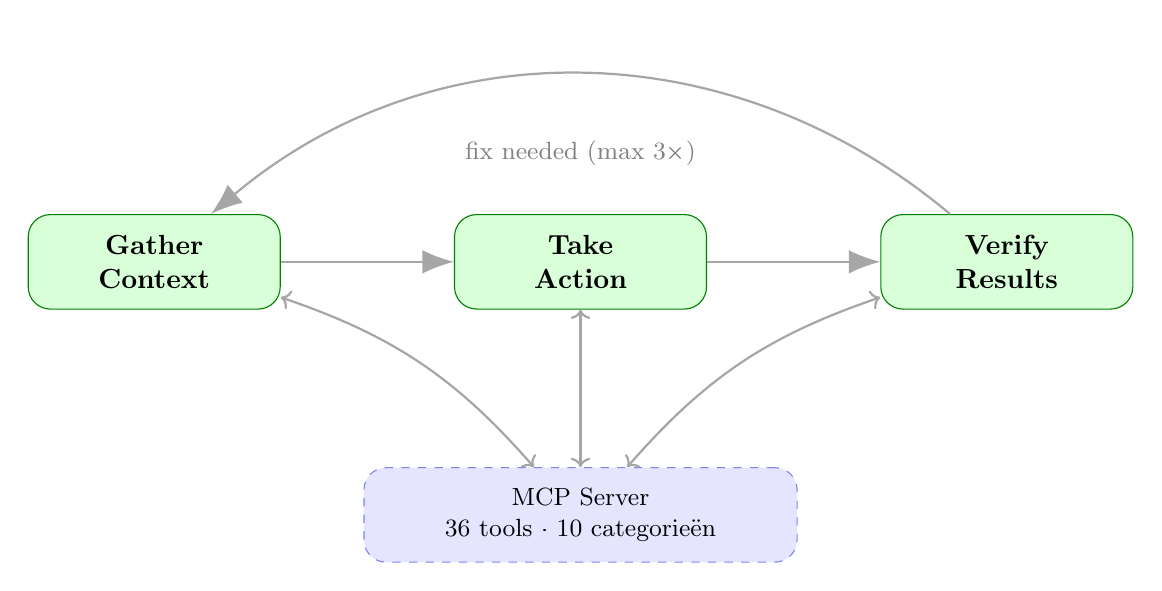
\begin{tikzpicture}[
  node distance=2.5cm,
  box/.style={
    draw, rounded corners=8pt,
    fill=green!15, draw=green!50!black,
    minimum width=3.2cm, minimum height=1.2cm,
    align=center, font=\normalsize\bfseries
  },
  mcp/.style={
    draw, dashed, rounded corners=8pt,
    fill=blue!10, draw=blue!50,
    minimum width=5.5cm, minimum height=1.2cm,
    align=center, font=\small
  },
  arr/.style={-{Latex[length=4mm, width=3mm]}, thick, draw=gray!70}
]
  \node[box] (gc) {Gather\\Context};
  \node[box, right=2.2cm of gc] (act) {Take\\Action};
  \node[box, right=2.2cm of act] (ver) {Verify\\Results};
  \node[mcp, below=2cm of act] (mcp) {MCP Server\\{\small 36 tools · 10 categorieën}};

  \draw[arr] (gc) -- (act);
  \draw[arr] (act) -- (ver);
  \draw[arr, bend right=40] (ver) to
    node[below, yshift=-0.7cm, font=\small, text=gray] {fix needed (max 3×)} (gc);
  \draw[arr, <->] (act) -- (mcp);
  \draw[arr, <->, bend left=15] (gc) to (mcp);
  \draw[arr, <->, bend right=15] (ver) to (mcp);
\end{tikzpicture}
\captionof{figure}{Cyclische Gather–Act–Verify lus via de MCP-server.}
\end{center}

\vfill

\section{Inner Dev Loop}

\begin{center}
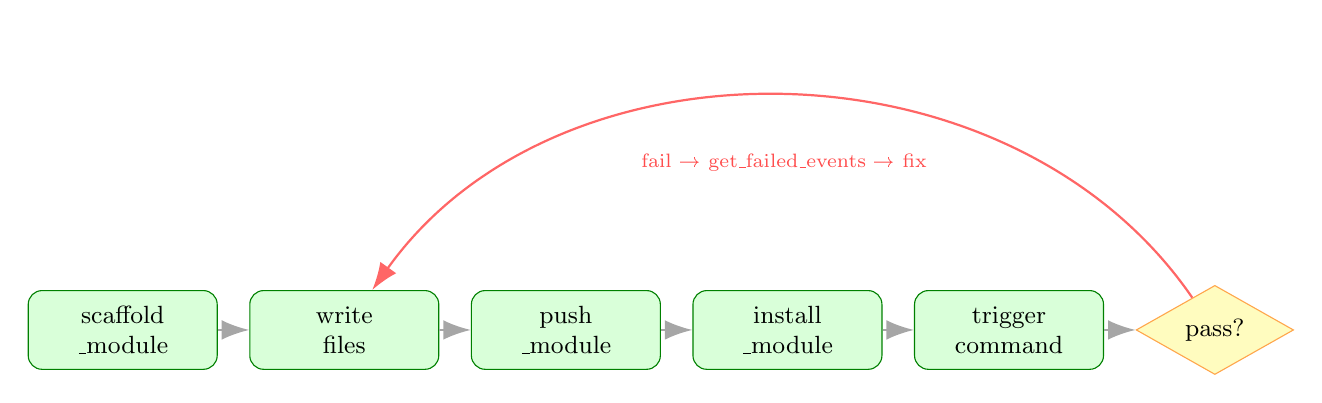
\begin{tikzpicture}[
  flowstep/.style={
    draw, rounded corners=5pt,
    fill=green!15, draw=green!50!black,
    minimum width=2.4cm, minimum height=1.0cm,
    align=center, font=\small
  },
  dec/.style={
    draw, diamond, aspect=1.6,
    fill=yellow!25, draw=orange!70,
    minimum width=2.0cm, minimum height=1.0cm,
    align=center, font=\small
  },
  arr/.style={-{Latex[length=3.5mm, width=2.5mm]}, thick, draw=gray!70}
]
  \node[flowstep] (sc) {scaffold\\\_module};
  \node[flowstep, right=0.4cm of sc] (wr) {write\\files};
  \node[flowstep, right=0.4cm of wr] (pu) {push\\\_module};
  \node[flowstep, right=0.4cm of pu] (in) {install\\\_module};
  \node[flowstep, right=0.4cm of in] (tr) {trigger\\command};
  \node[dec,  right=0.4cm of tr] (ok) {pass?};

  \draw[arr] (sc) -- (wr);
  \draw[arr] (wr) -- (pu);
  \draw[arr] (pu) -- (in);
  \draw[arr] (in) -- (tr);
  \draw[arr] (tr) -- (ok);

  \draw[arr, bend right=55, draw=red!60]
    (ok) to node[below, yshift=-0.6cm, font=\scriptsize, text=red!70]
    {fail → get\_failed\_events → fix} (wr);
\end{tikzpicture}
\captionof{figure}{Van scaffolding tot validatie op de live game server.}
\end{center}

\end{minipage}%
\hfill
\begin{minipage}[t][\postercolheight][s]{0.305\textwidth}

%-- KOLOM 2: Orchestratorarchitectuur · Methodologie · Resultaten -------------

\section{Orchestratorarchitectuur}
\vspace{1cm}
Bij $\geq$3 componenten spawnt de orchestrator parallelle subagents in geïsoleerde contextvensters.

\begin{center}
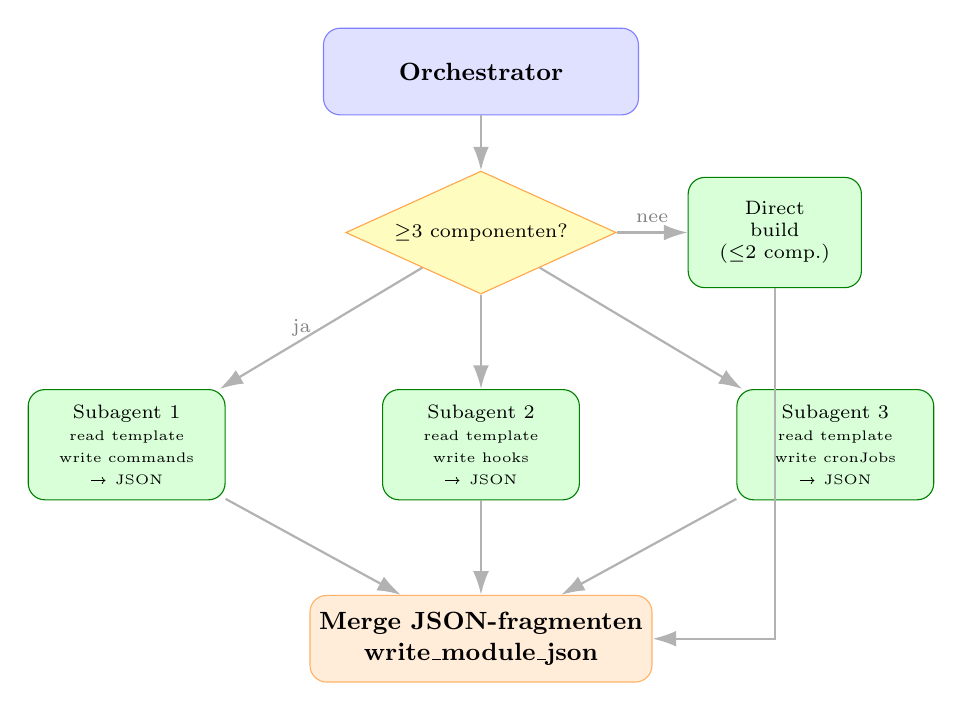
\begin{tikzpicture}[
  orch/.style={
    draw, rounded corners=6pt,
    fill=blue!12, draw=blue!50,
    minimum width=4.0cm, minimum height=1.1cm,
    align=center, font=\small\bfseries
  },
  sub/.style={
    draw, rounded corners=6pt,
    fill=green!15, draw=green!50!black,
    minimum width=2.5cm, minimum height=1.4cm,
    align=center, font=\scriptsize
  },
  merge/.style={
    draw, rounded corners=6pt,
    fill=orange!15, draw=orange!60,
    minimum width=4.0cm, minimum height=1.1cm,
    align=center, font=\small\bfseries
  },
  dec/.style={
    draw, diamond, aspect=2.2,
    fill=yellow!25, draw=orange!70,
    minimum width=3cm, minimum height=0.9cm,
    align=center, font=\scriptsize
  },
  arr/.style={-{Latex[length=3mm, width=2mm]}, thick, draw=gray!60}
]
  \node[orch] (orc) {Orchestrator};
  \node[dec, below=0.7cm of orc] (dec) {$\geq$3 componenten?};

  \node[sub, below=1.2cm of dec, xshift=-4.5cm] (sa1)
    {Subagent 1\\{\tiny read template}\\{\tiny write commands}\\{\tiny → JSON}};
  \node[sub, below=1.2cm of dec] (sa2)
    {Subagent 2\\{\tiny read template}\\{\tiny write hooks}\\{\tiny → JSON}};
  \node[sub, below=1.2cm of dec, xshift=4.5cm] (sa3)
    {Subagent 3\\{\tiny read template}\\{\tiny write cronJobs}\\{\tiny → JSON}};

  \node[merge, below=1.2cm of sa2] (mrg) {Merge JSON-fragmenten\\write\_module\_json};

  \node[sub, right=0.9cm of dec, minimum width=2.2cm] (direct)
    {Direct\\build\\($\leq$2 comp.)};

  \draw[arr] (orc) -- (dec);
  \draw[arr] (dec) -- node[left, font=\scriptsize, text=gray] {ja} (sa1);
  \draw[arr] (dec) -- (sa2);
  \draw[arr] (dec) -- (sa3);
  \draw[arr] (sa1) -- (mrg);
  \draw[arr] (sa2) -- (mrg);
  \draw[arr] (sa3) -- (mrg);
  \draw[arr] (dec) -- node[above, font=\scriptsize, text=gray] {nee} (direct);
  \draw[arr] (direct) |- (mrg);

\end{tikzpicture}
\captionof{figure}{Subagents werken parallel. De orchestrator voegt de JSON-fragmenten samen toe.}
\end{center}

\vspace{3cm}
\section{Resultaten}

\begin{center}
  \captionsetup{type=figure}
  
\includegraphics[width=1.0\linewidth]{fig_succes_zeroshot}
  \captionof{figure}{Totaal en zero-shot succes per model (van 11 modules).}
\end{center}

\begin{center}
  \captionsetup{type=figure}
  
\includegraphics[width=1.0\linewidth]{fig_shots_heatmap}
  \captionof{figure}{Correctiepogingen per module en model (1\,=\,zero-shot).}
\end{center}

\end{minipage}%
\hfill
\begin{minipage}[t][\postercolheight][s]{0.305\textwidth}

%-- KOLOM 3: Conclusies · Toekomstig onderzoek --------------------------------

\section{Methodologie}
\vspace{1cm}
\begin{center}
\renewcommand{\arraystretch}{1.4}
\begin{tabular}{cccc}
  {\LARGE\bfseries\color{hogent-blue}36}  &
  {\LARGE\bfseries\color{hogent-blue}11}  &
  {\LARGE\bfseries\color{hogent-blue}3}   &
  {\LARGE\bfseries\color{hogent-blue}31}  \\[2pt]
  \small tools & \small modules & \small modellen & \small metrics/run \\[12pt]
\end{tabular}

\medskip
\normalsize
\textbf{Modellen:} Claude Haiku 4.5 · Sonnet 4.6 · Opus 4.7\\[4pt]
\textbf{Aanpak:} Design science research\\[4pt]
\textbf{Observability:} Langfuse · fasetagging · promptcaching
\end{center}
\vspace{1cm}

\section{Conclusies}

\noindent\fcolorbox{hogent-darkgreen}{hogent-darkgreen!10}{%
  \parbox{\dimexpr\linewidth-2\fboxsep-2\fboxrule\relax}{%
    \medskip
    \normalsize\textbf{\textcolor{hogent-darkgreen}{$\checkmark$\ Gecorrigeerd inzicht}}\\[4pt]
    \small MCP \textbf{vervangt} documentatie niet,
    het structureert de aanbieding ervan efficiënt via promptcaching.
    \medskip
  }%
}

\begin{center}
\begin{tikzpicture}
  \fill[hogent-blue!20, rounded corners=5pt] (0,0) rectangle (0.9\linewidth,1.6);
  \fill[hogent-blue,    rounded corners=5pt] (0,0) rectangle (0.891\linewidth,1.6);
  \node[font=\normalsize\bfseries, text=white] at (0.45\linewidth,0.8)
    {$\approx$100\,\% cache-hit ratio};
  \node[font=\small, below=0.5cm] at (0.45\linewidth,0)
    {over alle 33 evaluatieruns};
\end{tikzpicture}
\end{center}

\begin{center}
  \captionsetup{type=figure}
  
\includegraphics[width=\linewidth]{fig_errors}
  \captionof{figure}{Gemiddeld aantal toolfouten per run.}
\end{center}

\begin{itemize}
  \item \textbf{Orchestrator-worker:} contextisolatie vermijdt contextpollutie
  \item \textbf{Architectuur $>$ model:} toolset-ontwerp en contextisolatie zijn
        bepalender dan modelkeuze
\end{itemize}
\vspace{3cm}

\section{Toekomstig onderzoek}
\vspace{1cm}
\begin{itemize}
  \item Overdraagbaarheid naar andere complexe API's
  \item Optimalisatie van het systeempromptontwerp
  \item Open-source modellen als vergelijking (Qwen, Llama)
  \item Embedding-gebaseerde clustering van foutpatronen
\end{itemize}

\end{minipage}

\end{document}
